%!TEX root = ../prak.tex
\section{Lab 9 Code Bloat bei Templates, Code Hoisting}
\subsection{Aufgabe 1: Untersuchung von Assemblercode bei Templates}

Die folgenden Optionen der GNU-Compiler könnten nützlich sein:

‐E \qquad  Precompile only, der Output wird auf stdout geschrieben\\
‐S \qquad Assembleroutput, ohne Objectfile erzeugen\\
‐c \qquad nur compilieren\\
‐O0\quad  keine Optimierung\\
‐O1\quad  Optimierungsstufe 1 (siehe g++ - Help für Details)\\
‐O2\quad  Optimierungsstufe 2\\
‐O3\quad  Optimierungsstufe 3\\
‐Os\quad  Optimierung auf Codegrösse\\

\textbf{Hinweis}
Jede Funktion in einem Objectfile oder Binary liegt an einer bestimmten Adresse und ist mit einem Symbol benannt, sofern im Debugmodus compiliert wurde. Mit dem Befehl nm [‐C] [objfile] kann der Inhalt einer solchen Datei ausgegeben werden. Mit der Option –C werden die Symbolnamen demangled. Siehe dazu auch die entsprechende man page.

\begin{enumerate}
  \item  Untersuchen Sie den Code im Verzeichnis ./Vorgabe/StackTemplate. Verschaffen Sie sich einen Überblick und werden Sie vertraut mit der Templateprogrammierung. Beachten Sie, dass einzelne Elementfunktionen implizit inline sind.
  \item Compilieren Sie den Code mit den Optimierungsstufen 0 und 3. Untersuchen Sie jeweils den entstandenen Assemblercode sowie die Codegrösse. Achten Sie vor allem darauf, ob die Funktionen aufgerufen werden (mit call) oder inline sind. Sind die Funktionen einfach oder mehrfach vorhanden?
  \item Ändern Sie den Code nun so ab, dass im Hauptprogramm ein zweiter int-Stack mit unterschiedlicher Grösse definiert wird. Compilieren Sie den Code wiederum unter Verwendung der Optimierungsstufen 0 und 3. Untersuchen Sie jeweils den entstandenen Assemblercode sowie die Codegrösse. Achten Sie darauf, ob die Funktionen aufgerufen werden (mit call) oder inline sind. Sind die Funktionen einfach oder mehrfach vorhanden?
\end{enumerate}

\subsubsection{Lösung}
Alle Programme wurden mit dem Compiler g++ v7.4.0 übersetzt.
\begin{enumerate}
  \item just do it.
  \item  Wenn mit Optimierungsstufe 0 compiliert wird, sind keine Elementfunktionen inline. Alle Elementfunktionen sind einfach vorhanden und werden mit call aufgerufen. Bei Optimierungstufe 3 sind sämtliche Funktionen der Klasse Stack inline. In der folgenden Tabelle sind die Codegrössen ersichtlich.
\begin{center}
  \begin{tabular}{c c c c c}
    \hline
    \hline
    Optimierung O… & g++ v4.7.3 Cygwin & g++ v4.8.4  & g++ v5.4.0 & g++ v7.4.0 \\
    \hline
    0 &
    61'738&
    13‘913&
    14‘024&
    13‘712\\
    3&
    60'043&
    13‘369&
    13‘480&
    13‘120\\
    \hline
    \hline
  \end{tabular}
\end{center}

  \item siehe ./Loesung/A1

\lstinputlisting[language=C++, style=C++, multicols=2]{900-Praktika/prak09/Loesung/A1/Stack.h}
\noindent\makebox[\linewidth]{\rule{\paperwidth}{0.4pt}}
\lstinputlisting[language=C++, style=C++, multicols=2]{900-Praktika/prak09/Loesung/A1/Stack.cpp}
\noindent\makebox[\linewidth]{\rule{\paperwidth}{0.4pt}}
\lstinputlisting[language=C++, style=C++, multicols=2]{900-Praktika/prak09/Loesung/A1/StackUI.h}
\noindent\makebox[\linewidth]{\rule{\paperwidth}{0.4pt}}
\lstinputlisting[language=C++, style=C++, multicols=2]{900-Praktika/prak09/Loesung/A1/StackUI.cpp}
\noindent\makebox[\linewidth]{\rule{\paperwidth}{0.4pt}}
\lstinputlisting[language=C++, style=C++, multicols=2]{900-Praktika/prak09/Loesung/A1/StackTest.cpp}

  Wenn ohne Optimierung compiliert wird, sind keine Elementfunktionen inline. Alle Elementfunktionen inklusive die Konstruktoren sind doppelt mit praktisch identischem Code vorhanden und werden mit call aufgerufen. Die Texte, die mit cout ausgegeben werden, sind nur einfach vorhanden.

\begin{lstlisting}[language=C++, style=C++, multicols=2]
Build mit -O0:
$ nm -C StackTest
...
0000000000000f90 W Stack<int, 3>::pop()
0000000000000f1e W Stack<int, 3>::push(int const&)
0000000000000ab2 W Stack<int, 3>::Stack()
0000000000000ab2 W Stack<int, 3>::Stack()
00000000000010c2 W Stack<int, 4>::pop()
0000000000001050 W Stack<int, 4>::push(int const&)
0000000000000ce8 W Stack<int, 4>::Stack()
0000000000000ce8 W Stack<int, 4>::Stack()
0000000000000ad0 W StackUI<int, 3>::dialog()
0000000000000a7a W StackUI<int, 3>::StackUI()
0000000000000a7a W StackUI<int, 3>::StackUI()
0000000000000d06 W StackUI<int, 4>::dialog()
0000000000000a96 W StackUI<int, 4>::StackUI()
0000000000000a96 W StackUI<int, 4>::StackUI()
0000000000000fec W Stack<int, 3>::peek() const
0000000000001182 W Stack<int, 3>::isFull() const
000000000000103a W Stack<int, 3>::isEmpty() const
0000000000000f7e W Stack<int, 3>::wasError() const
000000000000111e W Stack<int, 4>::peek() const
000000000000119a W Stack<int, 4>::isFull() const
000000000000116c W Stack<int, 4>::isEmpty() const
00000000000010b0 W Stack<int, 4>::wasError() const
...


Build mit -O3:
$ nm -C StackTest
...
0000000000000a80 W StackUI<int, 3>::dialog()
0000000000000d50 W StackUI<int, 4>::dialog()
...
\end{lstlisting}
  Bei älteren Compilerversionen (z.B. g++-Version v3.4.4) waren mit Optimierungstufe 3 nur die impliziten inline-Elementfunktionen inline. Alle weiteren Elementfunktionen waren ebenfalls doppelt vorhanden und wurden mit call aufgerufen. Wenn hingegen g++ v4.8.4, g++ v5.4.0 oder g++ v7.4.0 genommen wird, sind alle Elementfunktionen ausser \texttt{StackUI::dialog()} inline. Diese Funktion ist dann zweifach vorhanden, je für einen Stack der Grösse 3 und der Grösse 4, und wird wie folgt aufgerufen:

\begin{lstlisting}[language=C++, style=C++]
call _ZN7StackUIIiLi3EE6dialogEv
...
call _ZN7StackUIIiLi4EE6dialogEv
\end{lstlisting}
In der folgenden Tabelle sind die Codegrössen ersichtlich.
\begin{center}
  \begin{tabular}{c c c c c}
    \hline
    \hline
    Optimierung O… & g++ v4.7.3 Cygwin & g++ v4.8.4  & g++ v5.4.0 & g++ v7.4.0 \\
    \hline
    0 &
66'052&
14‘440&
14‘544&
14‘240\\
3&
61'389&
13‘420&
13‘528&
13‘168\\
    \hline
    \hline
  \end{tabular}
\end{center}
\end{enumerate}

\subsection{Aufgabe 2: Verhindern von Code Bloat durch Code Hoisting}
In dieser Aufgabe soll untersucht werden, wie mittels Code Hoisting der bei Templates häufig entstehende Code Bloat vermieden werden kann. Die heutigen Compiler erzeugen zwar immer besseren Code. Es ist trotzdem sinnvoll, mittels Code Hoisting möglichen Code Bloat zu vermeiden.

Die Klasse \texttt{StackUI} lassen wir unverändert. Analysieren Sie, welche Teile in der Klasse \texttt{Stack} unabhängig von der Grösse sind. Lagern Sie alle diese Teile in eine Basisklasse aus. Compilieren Sie den Code wiederum mit den Optimierungsstufen 0 und 3. Untersuchen Sie jeweils den entstandenen Assemblercode. Achten Sie darauf, ob die Funktionen aufgerufen werden (mit \texttt{call}) oder inline sind. Sind die Funktionen einfach oder mehrfach vorhanden?

\subsubsection{Lösung}
Code hoisting, siehe ./Loesung/A2. Beachten Sie auch die Kommentare im Source Code.

In der Klasse Stack sollen alle von der Grösse unabhängigen Teile in eine Basisklasse ausgelagert werden. Die Analyse, was unabhängig von der Grösse ist, ist nicht so trivial. Sind beispielsweise die Elementfunktionen isEmpty() und isFull() unabhängig von der Grösse oder nicht? Weiss man das bereits bei der Deklaration oder ist es erst bei der Implementation bekannt? Aus der Implementation geht hervor, dass die Methode isEmpty() unabhängig ist, isFull() jedoch nicht. Alle weiteren Elementfunktionen, die isFull() benötigen, sind demnach auch nicht unabhängig, das ist z.B. push().

Damit die Unterklassen einfach auf die Attribute zugreifen können, sollten top und error als protected statt private definiert werden. In der Basisklasse ist der Array elems[] nicht bekannt, da dieser ja eben abhängig von der Grösse ist. Also müssten beinahe alle Elementfunktionen (alle, die auf den Array zugreifen) in die Unterklasse. Um das zu verhindern, kann im Ctor der Basisklasse ein Pointer auf den elems-Array gesetzt werden. In der Basisklasse wird dann damit gearbeitet. Dies ist zwar nicht gerade schön, allerdings löst es den Code Bloat. Man beachte, dass der Ctor von StackNoSize protected gesetzt wird, damit nur eine Unterklasse diesen aufrufen kann.

Wenn ohne Optimierung compiliert wird, sind keine Elementfunktionen inline. Alle Elementfunktionen und Konstruktoren der Basisklasse sind nur noch einfach vorhanden, alle anderen Elementfunktionen sind doppelt vorhanden
.
Bei älteren Compilerversionen (z.B. g++-Version v3.4.4) waren mit Optimierungstufe 3 die impliziten inline-Elementfunktionen inline. Funktionen der Basisklasse waren nur noch einfach, alle anderen Funktionen doppelt vorhanden. Wenn hingegen g++ v7.4.0 genommen wird, sind alle Elementfunktionen ausser StackUI::dialog() inline. Diese Funktion ist dann zweifach vorhanden, je für einen Stack der Grösse 3 und der Grösse 4.

\lstinputlisting[language=C++, style=C++, multicols=2]{900-Praktika/prak09/Loesung/A2/Stack.h}
\noindent\makebox[\linewidth]{\rule{\paperwidth}{0.4pt}}
\lstinputlisting[language=C++, style=C++, multicols=2]{900-Praktika/prak09/Loesung/A2/Stack.cpp}
\noindent\makebox[\linewidth]{\rule{\paperwidth}{0.4pt}}
\lstinputlisting[language=C++, style=C++, multicols=2]{900-Praktika/prak09/Loesung/A2/StackNoSize.h}
\noindent\makebox[\linewidth]{\rule{\paperwidth}{0.4pt}}
\lstinputlisting[language=C++, style=C++, multicols=2]{900-Praktika/prak09/Loesung/A2/StackNoSize.cpp}
\noindent\makebox[\linewidth]{\rule{\paperwidth}{0.4pt}}
\lstinputlisting[language=C++, style=C++, multicols=2]{900-Praktika/prak09/Loesung/A2/StackUI.h}
\noindent\makebox[\linewidth]{\rule{\paperwidth}{0.4pt}}
\lstinputlisting[language=C++, style=C++, multicols=2]{900-Praktika/prak09/Loesung/A2/StackUI.cpp}
\noindent\makebox[\linewidth]{\rule{\paperwidth}{0.4pt}}
\lstinputlisting[language=C++, style=C++, multicols=2]{900-Praktika/prak09/Loesung/A2/StackTest.cpp}

\begin{center}
  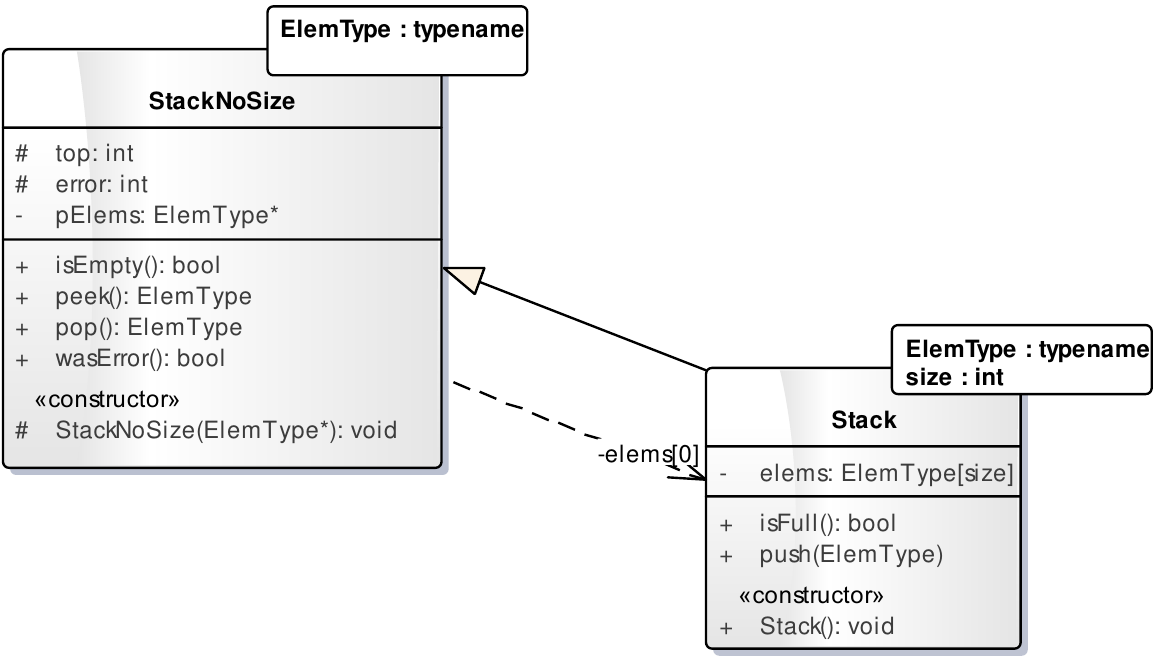
\includegraphics[width=.6\linewidth]{900-Praktika/prak09/1.PNG}
\end{center}
